\begin{exercise}{
    Consider the following abstract domain $Sign_k$ of $\left<\wp(\Z), \subseteq\right>$ where $k \in \Z$ is any given integer:
    \begin{center}
        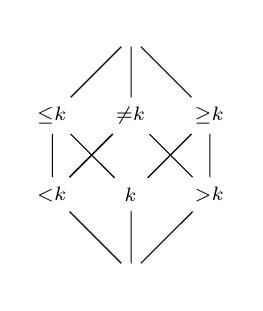
\begin{tikzpicture}
            \node (top) at (1, 3) {$\Z$};
            \node (leq) at (0, 2) {$\Z_{\leq k}$};
            \node (neq) at (1, 2) {$\Z_{\neq k}$};
            \node (geq) at (2, 2) {$\Z_{\geq k}$};
            \node (lt) at (0, 1) {$\Z_{< k}$};
            \node (eq) at (1, 1) {$\Z_{k}$};
            \node (gt) at (2, 1) {$\Z_{> k}$};
            \node (bot) at (1, 0) {$\varnothing$};

            \draw (top) -- (leq) -- (eq) -- (bot);
            \draw (top) -- (neq) -- (lt) -- (bot);
            \draw (top) -- (geq) -- (gt) -- (bot);
            \draw (leq) -- (lt) -- (neq) -- (gt);
            \draw (geq) -- (eq);
        \end{tikzpicture}
    \end{center}
    Hence, $Sign_k$ is a parametric abstract domain of signs, where the constant 0 is replaced by any integer parameter $k \in \Z$. Provide sound definitions for the following abstract transfer functions: $\Bsharp{x \leq k}$, $\Asharp{x * y}$, $\Asharp{x / k}$, $\Asharp{x - y}$, which are as precise as possible, ideally the best correct approximation.
}
    
\end{exercise}
